\documentclass[a4paper, 12pt, titlepage]{report}

\usepackage[english]{babel}
\usepackage{listings}
\usepackage{setspace}
\usepackage{color}
\usepackage{mathptmx}
\usepackage{titlesec}
\usepackage{lipsum}
\usepackage{graphicx}
\usepackage[dvipsnames]{xcolor}
\usepackage{hyperref}

\newcommand{\emptypage}{\newpage\shipout\null}
\newcommand{\autori}[1]{\textsc{\texttt{#1}}}
\lstset
{
	basicstyle=\scriptsize\ttfamily,keywordstyle=\color{OliveGreen},
	commentstyle=\color{blue},stringstyle=\color{red},showstringspaces=false,
   	breaklines=true,tabsize=4, frame=single, rulecolor=\color{black}
}

\newenvironment{dedication}
  {\clearpage           % we want a new page
   \thispagestyle{empty}% no header and footer
   \vspace*{\stretch{1}}% some space at the top 
   \itshape             % the text is in italics
   \raggedleft          % flush to the right margin
  }
  {\par % end the paragraph
   \vspace{\stretch{3}} % space at bottom is three times that at the top
   \clearpage           % finish off the page
  }
 
\renewcommand\labelitemii{--}

\begin{document}

\begin{titlepage}
High performance networking extensions for VirtualBox
\end{titlepage}

\emptypage

\begin{dedication}
Alla mia famiglia,\\
a Erika,\\
ai miei amici.
\end{dedication}

\begin{abstract}
Virtual Machine systems are commonly used in several organizations providing network services, since those systems supply high reliability, security and availability. Therefore, network performance has become a critical issue to deal with, since Virtual Machine systems are widespread nowadays.
\\
\\
In this thesis we are going to present VirtualBox~\cite{vbox} hypervisor, giving some details about its architecture and analyzing network performances of the existing solution. We then implement an extension that interfaces the hypervisor with netmap framework~\cite{netmap}, which provides fast packet I/O. Finally, we present some optimizations to an emulated network device (e1000 in our case), that considerably improve network performances.
\end{abstract}
\emptypage
\tableofcontents

\chapter{Introduction}

It is important to point out that the term \textit{Virtual Machine} may have multiple interpretations, so we must first specify which one of those meanings we are referring to.

When we talk about Virtual Machine (VM), we refer to a \textit{virtualized} computing environment running on top of a physical computing environment; as a result, we get one or more independent VMs, which may be different from the original one.\newline
Before proceeding, we introduce some terminology:
\begin{itemize}
\item \textit{Guest}: The VM.
\item \textit{Host}: The physical computing environment that \textit{hosts} one or more VMs.
\item \textit{Virtual Machine Monitor (VMM)}: The software part that provides support for virtualization. Also known as \textit{Hypervisor}.
\end{itemize}

The main reason that caused the spread of VMs is the abstraction levels that it introduces; this brings many benefits:
\begin{itemize}
\item \textit{Flexibility}: you can run programs compiled for a given Instruction Set Architecture (ISA) and/or a given Operating System (OS) on top of a computer that has a different ISA and/or different OS (e.g. you can test new software on different architectures without \textbf{having} one machine per architecture).
\item \textit{Protection}: each guest is \textbf{isolated}, which means that you can execute different applications on different VMs, so that if an application has a security issue, only the VM (or VMs) running that specific software will be exposed to it.
\item \textit{Resources usage}: one single physical machine may provide multiple services using the 100\% of the resources, instead of using many underutilized physical machines, thus reducing costs and saving energy.
\item \textit{Mobility}: replicating VMs to other locations is only a matter of copying/transmitting some files; this helps avoiding multiple setups since through a VM you can bring a functioning computing environment ready to use to the user.
\end{itemize}

As stated before, the term \textit{Virtual Machine} may have several meanings. A generic architecture of the "class" of VMs we will refer to (called \textit{Type 2 System Virtual Machines}), is shown in figure 1.1. In this case the VMM is a regular OS process, that runs in the host OS along with other processes. The VMM can access the physical resources through the OS services, which depend on the specific OS. We will not investigate other classes of Virtual Machines since this topic falls outside this work. 
\begin{figure}[!h]
	\centering
	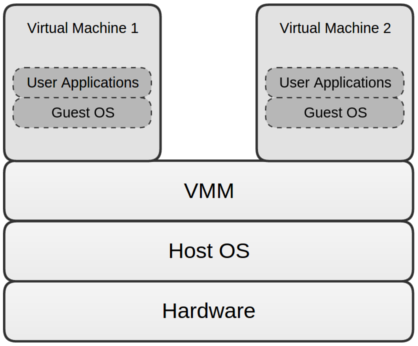
\includegraphics[scale=0.5]{img/vm_arch.png}
	\caption{Type 2 System Virtual Machine generic architecture}
\end{figure}

\section{Virtual Machine Implementation}
The basic idea behind VMs, is to \textit{emulate}, i.e. to execute code written for a certain environment, using another environment. In the following, we will briefly present the three basic techniques to implement emulation: interpretation, dynamic translation, hardware-based virtualization.
\subsection{Interpretation}
This is the naive emulation technique. The VMM has to perform in software what a physical CPU would have done in hardware: so it will be implemented as a loop, for each iteration, performs  the fetch, decode and execute phases of instruction execution.
\\
\\
Writing an interpreter for a modern ISA can be a very long and difficult process, even if it is conceptually simple; in fact, it is just a matter of reading an Instruction Set specification and implement all the possible instructions respecting the specifications.\\
However, the simplicity of this approach is responsible for its inefficiency; as a matter of fact, for each source instruction, the VMM has to execute many host instructions (e.g. 30-100) to perform in software all the necessary operations. The average \textit{translation ratio} is very high (e.g. 40).
\subsection{Dynamic translation} \label{subsec:dyn_tr}
This is a more sophisticated form of emulation. Rather than performing a "source-code-to-source-code" translation, the idea is to translate it into an equivalent binary code that can be executed directly on the host CPU.\\
This method amortizes the cost of interpretation, doing the fetch and decode phases only once or a few times. The code execution step of an instruction or a block of instructions is generated once (or a few times) and stored in a \textit{Code Cache}. After some time the code cache will contain the complete translation of the source program into the host ISA.\newline
As a result, the average translation ratio can be close to 1, giving an acceptable performance.
\\
\\
This technique is way more complicated than the previous one. In this case, several problems are present:
\begin{itemize}
\item \textit{code-discovery}: makes impossible to do static translation
\item \textit{code-location}: different address space of the guest and host systems
\item \textit{state mapping}: the way the VMM maps guest registers and the like to the host ones
\end{itemize}

It is interesting to notice that both interpretation and dynamic translation can make sense also in the case that guest and host have the same ISA; if this is the case, the translation is simplified since the code can be natively executed on the host machine, without performance losses.\\
However there are some cases where emulation in software my be necessary. As a typical example, memory accesses to the I/O space may need software emulation. In particular, if the guest wants to access a physical resource that is present on the host (e.g. a network adapter), the VMM cannot allow direct access to the device, because other processes could be accessing the same device at the same time, and, obviously, the host network driver and the guest network driver are not aware of each other. On the other hand, if the guest wants to access a virtual device (which does not exist on the host), the I/O instruction must be \textit{trapped}\footnote{Guest execution is interrupted and the VMM takes control.} in order to emulate the device behavior in software.

\subsection{Hardware-based virtualization} \label{subsec:hw_virt}
Due to the widespread use of VMs, extensions for virtualization were introduced by processor vendors. Thanks to these hardware assists, some of the problems affecting dynamic translation techniques have been overcome, and at the same time they have made it easier to execute guest code natively. Both AMD and Intel proposed their extensions for the x86 ISA, AMD-v (\cite{amd-v}) and VT-x (\cite{vt-x}) respectively.
\\
\\
With this new extension, the CPU can execute in two different modes: \textit{root mode} and \textit{VM mode} (or \textit{non-root mode}). The CPU can switch from root mode to VM mode through a so called \textit{VM entry} instruction, while can switch back to root mode through a so called \textit{VM exit} instruction. When in VM mode, the CPU can execute guest code in a controlled environment, i.e. the CPU cannot execute some safety-critical instructions (e.g. I/O instructions); when necessary, CPU performs a VM exit and runs host code (VMM or other processes). The switch operation between host world and guest world is similar to a context switch, since it involves the saving of the host state and loading the guest state (and vice versa). Although performed in hardware, these transitions between host and guest worlds are expensive in terms of performance, because software overhead, OS operations and userspace/kernelspace transitions are involved in the switching operations, but they are also necessary when dealing with I/O operations or interrupts. Hence, VM switches must be minimized in order to achieve good I/O performances.
\section{I/O Virtualization techniques}
Emulating a device means doing in software what the device would do in hardware. Thus, when a guest accesses an I/O device (e.g. writes to a device register), the VMM must take over and emulate all the operations associated with the specific I/O access.
\\
\\
In order to improve I/O virtualization techniques, three approaches have been defined:
\begin{itemize}
\item Hardware support in the devices (\textit{virtual functions} and IOMMU \cite{iommu}), so that a guest can directly access devices in a protected way and run at native speed.
\item Runtime optimizations in VMM. E.g. running short code involving multiple I/O instructions in interpreted mode saves some VM exits\footnote{See \cite{vmm_opt} for details.}.
\item Design \textit{virtual} device models in order to reduce expensive operations in device emulations (e.g. I/O accesses and interrupts). This approach is known as \textit{device paravirtualization} and produced some virtual device models, such as VirtIO (\cite{virtio}).
This requires synchronization and memory sharing between the guest and VMM in order to exchange information, while interrupts are used only for notification purposes. In that way it is easier to minimize the amount of VM exits.
\end{itemize}
\chapter{VirtualBox}
In this chapter we will present VirtualBox hypervisor, giving details about its features (section~\ref{sec:features}), its internal architecture (section~\ref{sec:architecture}), and how the behavior of e1000 device is emulated (section~\ref{sec:e1000_emu}).
\\
As host OS, we used Ubuntu 15.10 64-bit with kernel version 4.2.0. The guest OS is generally the same as the host OS host, but some tests have been performed with FreeBSD as guest too.


\section{VirtualBox features} \label{sec:features}
VirtualBox is a free, open source and cross-platform type 2 VMM, so it is able to run an arbitrary OS, regardless of the host OS, and it is implemented as a regular process in the host OS, therefore it can make use of all OS services. At the time of the writing, VirtualBox version number is 5.0.4, so we will refer to that version for Linux OS (since our host OS is Linux based).
\\
\\
Here is a brief outline of VirtualBox main features:
\begin{itemize}
\item \textbf{Portability.} VirtualBox runs on a large number of a 32-bit and 64-bit host operating systems. It can run VMs created on different hosts and/or with different virtualization software.
\item \textbf{Multiple virtualization interfaces.} VirtualBox provides three different virtualization interfaces
	\begin{itemize}
	\item \textit{Minimal}: Announces the presence of a virtualized environment.
	\item \textit{KVM}: Presents a Linux KVM hypervisor interface which is recognized by Linux kernels starting with version 2.6.25.
	\item \textit{Hyper-V}: Presents a Microsoft Hyper-V hypervisor interface which is recognized by Windows 7 and newer operating systems.
	\end{itemize}
We chose the KVM interface for tests and implementations.
\item \textbf{No hardware virtualization required.} Even if hardware virtualization is fully supported, VirtualBox does not require the processor features such as Intel VT-x or AMD-V; in that way VirtualBox can be used also on old hardware which has not these features.
\item \textbf{Guest Additions.} VirtualBox Guest Additions are software package which can be installed \textit{inside} of supported guest systems to provide additional integration and communication with the host system (e.g. accelerated 3D graphics, automatic adjustment of video resolution and more).
\item \textbf{Great hardware support.} Among others, VirtualBox supports:
	\begin{itemize}
	\item \textbf{Guest multiprocessing (SMP).} VirtualBox can present up to 32 virtual CPUs to each virtual machine, regardless of how many CPU cores are physically present on the host.
	\item \textbf{USB device support}. VirtualBox implements a virtual USB controller that allows to connect arbitrary USB devices to VMs without having to install device-specific drivers on the host.
	\item \textbf{Hardware compatibility.} VirtualBox virtualizes a vast array of virtual devices. That includes IDE, SCSI and SATA hard disk controllers, several virtual network cards (including e1000) and so on.
	\item \textbf{Full ACPI support.} The Advanced Configuration and Power Interface (ACPI) is fully supported by VirtualBox.
	\end{itemize}
\item \textbf{Multigeneration branched snapshots.} VirtualBox can save arbitrary snapshots of the state of the VM. You can go back in time and revert the VM to any such snapshot and start an alternative VM configuration from there, effectively creating a whole snapshot tree.
\item \textbf{VM groups.} VirtualBox provides a groups feature that enables the user to organize and control VMs collectively, as well as individually.
\item \textbf{Clean and modular architecture.} VirtualBox has an extremely modular design with well-defined internal programming interfaces and clean separation of client and server code (i.e. code related to VMs and code related to the VMM, respectively).
\end{itemize}
\section{VirtualBox architecture} \label{sec:architecture}
In this section we will present the internal architecture of VirtualBox, giving details about its implementation that is necessary to understand in order to implement our optimizations.
\subsection{VirtualBox kernel modules}
VirtualBox provides different kernel modules that the user should add to the host kernel:
\begin{itemize}
\item \textit{vboxdrv}: The only mandatory module. This is needed by the VMM to gain control over the host system. It is used to manage the host/guest world switches and device emulations.
\item \textit{vboxnetadp}: "vboxnetadp" stands for "VirtualBox Network Adapter". It is needed to create a host networking interface (called \textit{vboxnet}); that interface (basically a virtual switch), is used to connect VMs to each other (and/or to the host). It is necessary when VirtualBox networking mode is set on \textbf{host-only} or \textbf{bridged} (these modes will be explained in section~\ref{subsec:net_modes}).
\item \textit{vboxnetflt}: "vboxnetflt" stands for "VirtualBox Network Filter". It is a kernel module that attaches to a real interface on the host and filters and injects packets. As for vboxnetadp, it is only necessary for host-only and bridged modes.
\item \textit{vboxpci}: This kernel module provides PCI card passthrough. This is used when the user wants to use a PCI device on the guest, even if the related driver is not available on the host.
\end{itemize}
\subsection{Software Virtualization}
As stated in section~\ref{sec:features}, VirtualBox fully supports hardware virtualization. However, since this is not a requirement, in the event that hardware virtualization is not present, VirtualBox makes use of a technique defined as \textit{Software virtualization}.
In order to understand the software virtualization technique, it is important to understand how CPUs provide a mechanism of protection at microcode level called \textit{Protection rings}.
\subsubsection{Privilege rings}
\begin{figure}[!h]
	\centering
	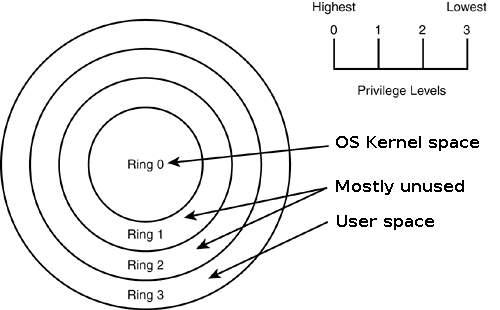
\includegraphics[scale=0.5]{img/rings.png}
	\caption{Protection rings}
\end{figure}
As shown in figure 2.1, there are four privilege levels or \textit{rings}, numbered from 0 to 3, with ring 0 (R0) being the most privileged and ring 3 (R3) being the least. The use of ring allows for system software to restrict task from accessing data or executing privileged instructions. In most environments, the OS and some device drivers run in R0 and applications run in ring 3~\cite{rings}.
\subsubsection{Software Virtualization}
In addition to the four privilege rings provided bu the hardware, we need to differentiate between \textit{host context} and \textit{guest context}.
\begin{itemize}
\item In \textit{host context}, everything is as if no VMM was active. This might be the active mode if another application on the host has been scheduled CPU time; in that case, there is a host R3 mode and a host R0 mode.
\item In \textit{guest context} a VM is active. So long as the guest code is running in ring 3, this is not much of a problem since a hypervisor can set up the page tables properly and run that code natively on the processor. The problems mostly lie in how to intercept what the guest's kernel does.
\end{itemize}
When starting a VM, through its R0 support kernel driver, VirtualBox has set up the host system so that it can run most of the guest code natively, but it inserted itself at the "bottom" of the picture. It can then assume control when needed, e.g. if a privileged instruction is executed, the guest \textit{traps}; VirtualBox may then handle this and either route a request to a virtual device or possibly delegate handling such things to the guest or host OS. In guest context, VirtualBox can therefore be in one of three states:
\begin{itemize}
\item Guest R3 code is run unmodified, at full speed, as much as possible. The number of faults will generally be low. This is also referred to as \textit{raw mode}, as the guest R3 code runs unmodified.
\item For guest code in R0, VirtualBox employs a trick: it actually reconfigures the guest so that its R0 code is run in \textbf{ring-1} (R1) instead. As a result, when guest R0 code (actually running in R1) such as a guest device driver attempts to write to an I/O register or execute a privileged instruction, the VirtualBox hypervisor in "real" R0 can take over.
\item The VMM can be active. Every time a fault occurs, VirtualBox looks at the offending instruction and can relegate it to a virtual device, the host OS, the guest OS, or run it in the \textbf{recompiler}.
\\
\\
In particular, the recompiler is used when guest code disables interrupts and VirtualBox cannot figure out when they will be switched back on. The recompiler is based on the dynamic translation technique (section~\ref{subsec:dyn_tr}).
\end{itemize}
Unfortunately this only wokrs to a degree. Among others, the following situations require special handling:
\begin{enumerate}
\item Running R0 code in R1 causes a lot of additional instruction faults, as R1 is not allowed to execute any privileged instructions (of which guest's R0 contains plenty). With each of these faults, the VMM must step in and emulate the code to achieve the desired behavior. While this works, emulating thousands of these faults is very expensive and severely hurts the performance of the virtualized guest.
\item There are certain flaws in the implementation of R1 in the x86 architecture that were never fixed. Certain instructions that \textit{should} trap in R1 don't. If the guest is allowed to execute these, it will see the true state of the CPU, not the virtualized state.
\item A hypervisor typically needs to reserve some portion of the guest's address space for its own use. This is not entirely transparent to the guest OS and may cause clashes.
\item The SYSENTER instruction (used for system calls) executed by an application running in a guest OS always transitions to R0. But that is where the VMM runs, not the guest OS. In this case, the hypervisor must trap and emulate the instruction even when it is not desirable.
\item The CPU segment registers contain a "hidden" descriptor cache which is not software-accessible. The hypervisor cannot read, save or restore this state, but guest OS may use it.
\item Some resources must (and can) be trapped by the hypervisor, but the access is so frequent that this creates a significant performance overhead.
\end{enumerate}
To fix these performance and security issues, VirtualBox contains a \textit{Code Scanning and Analysis Manager} (CSAM), which disassembles guest code, and the \textit{Patch Manager} (PATM), which can replace it at runtime.
\\
\\
Before executing R0 code, CSAM scans it recursively to discover problematic instructions. PATM the performs \textit{in-situ} patching, i.e. it replaces the instruction with a jump to hypervisor memory where an integrated code generator has places a more suitable implementation. In reality, this is a very complex task as there are lots of odd situations to be discovered and handled correctly.
\\
\\
In addition, every time a fault occurs, VirtualBox analyzes the offending code to determine if it is possible to patch it in order to prevent it from causing more faults in the future. This approach works well in practice and dramatically improves software virtualization performance.
\subsection{Hardware virtualization}
As stated in section~\ref{subsec:hw_virt}, with Intel VT-x there are two distinct modes of CPU operation: root mode and non-root mode.
\begin{itemize}
\item In root mode, the CPU operates much like older generations of processors without VT-x support. There are four privilege rings, and the same instruction set is supported, with the addition of several virtualization specific instructions. Root mode is what a host operating system without virtualziation uses, and it is also used by a hypervisor when virtualization is active.
\item In non-root mode, CPU operation is significantly different. There are still four privilege rings and the same instruction set, but a new structure called \textit{Virtual Machine Control Structure} (VMCS) now controls the CPU operation and determines how certain instructions behave. Non-root mode is where guest systems run.
\end{itemize}
The VMCS includes a guest and host state area which is saved/restored when switching between the two modes (\textit{VM entry} and \textit{VM exit}). Most importantly, the VMCS controls which guest operations will cause VM exits.
Thanks to the VMCS, a hypervisor can allow a guest to write certain bits in shadowed control registers,but not others. This enables efficient virtualziation in cases where guests can be allowed to write control bits without disrupting the hypervisor, while preventing them from altering control bits over which the VMM needs to retain full control. The VMCS also provides control over interrupt delivery and exceptions.
\\
\\
Whenever an instruction or event causes a VM exit, the VMCS contains information about the exit reason. Thus the hypervisor can efficiently handle the condition without needing advanced techniques such as CSAM and PATM described above.
\\
\\
VT-x inherently avoids several of the problems which software virtualization faces. The guest has its own completely separate address space not shared with the hypervisor, which eliminates potential clashes. Additionally, guest OS kernel code runs at privilege R0 in non-root mode, obviating the problems by running R0 code at less privileged levels. Naturally, even at R0 in non-root mode, any I/O access by guest code still causes a VM exit, allowing for device emulation.
\\
\\
We restrict our work to the Hardware Virtualization solutions, because the optimizations we introduce are effective in limiting the amount of switches between root mode and non-root mode.
\subsection{Emulation Threads} \label{subsec:EMT}
When a VM is started, a user-defined number of SMP processors is assigned to the VM itself. Each CPU is emulated through a so called \textit{Emulation Thread} (EMT), so we have one EMT per SMP processor. An EMT is responsible of executing guest code, emulating devices and handle the transition between host world and guest world. 
\\
When using hardware virtualization (as we stated before, this is our case), an EMT continuously switches between root mode and VM mode (see section~\ref{subsec:hw_virt}).
\\
\\
Let us assume that the EMT is running guest code, e.g. an application. At some point, the application tries to execute an I/O operation, causing a SYSENTER instruction in the guest. Therefore, the CPU executing the EMT, switches from R3 to R0 (still in VM mode), in order to run the guest kernel code. At this point, the "true" I/O operation (such as a write operation in a register) produces a VM exit, so the CPU switches from VM mode to root mode. On a VM exit the EMT stops executing guest code and start executing VirtualBox code (in kernelspace), in order to handle the event that caused the VM exit itself. Handling a VM exit \textit{may} cause the EMT to execute userspace code in order to emulate a device, switching back to kernelspace after the device emulation (more on this in section~\ref{sec:e1000_emu}). After the event has been handled, the EMT executes a VM entry (i.e. CPU switches back to VM mode) and continues to run guest code from the point where it was interrupted.
\\
\\
\begin{figure}[!ht]
	\centering
	 	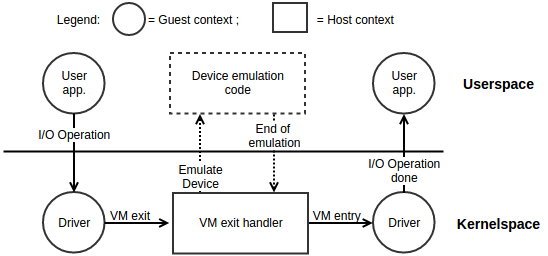
\includegraphics[scale=.75]{img/emt_flow.png}
	 	\caption{Example of EMT execution flow}
	 	\label{img:emt_flow}
\end{figure}
Figure~\ref{img:emt_flow} shows the situation described above.
\subsection{Networking modes} \label{subsec:net_modes}
For a VM it is fundamental to communicate to the outside world using the networking infrastructure, otherwise the VM becomes useless.
\\
Nevertheless, a VM is "just" a software entity, so it is not connected to any \textit{real} network. Therefore the VMM must provide some kind of virtualized network infrastructure, so that guest OS thinks its \textbf{virtual} network device is connected to a \textbf{physical} network and can then exchange packets with the outside.
\\
\\
VirtualBox provides several of these network infrastructures called \textit{Networking modes}; in that way a user can choose the most suitable way to connect her VM. Among the others, the main network modes provided by VirtualBox are the following:
\begin{itemize}
\item \textbf{Not attached} In this mode, VirtualBox reports to the guest that a network card is present, but there is no connection, as if no Ethernet cable was plugged into the card.
\item \textbf{Network Address Translation (NAT)} A VM with NAT enabled acts much like a real computer that connects to the Internet through a router. The "router", in this case, is the VirtualBox networking engine, which maps traffic from and to the VM transparently. In VirtualBox this router is placed between each VM and the host.
\\
The VM  receives its network address and configuration on the private network from a DHCP server integrated into VirtualBox. The IP address thus assigned to the VM is usually on a completely different network than the host.

\item \textbf{Bridged networking} With bridged networking, VirtualBox uses a device driver on the host system (\textit{vboxnetflt} kernel module) that filters data from the physical network adapter. That is why it is called "network filter" driver. This allows VirtualBox to intercept data from the physical network and inject data into it, effectively creating a new network interface in software. When a guest is using such a new software interface, it looks to the host system as though the guest were physically connected to the interface using a network cable: the host can send data to the guest through that interface and receive data from it. This means that the user can set up routing or bridging between the guest and the rest of the network.
\item \textbf{Internal networking} It is similar to bridged networking in that the VM can directly communicate with the outside world. However, the "outside world" is limited to other VMs on the same host which connect to the same internal network, which is identified simply by its name.
\\
Even though technically, everything that can be done using internal networking can also be done using bridged networking, there are security advantages with internal networking. In bridged mode, all traffic goes through a physical interface of the host system. It is therefore possible to attach a packet sniffer to the host interface and log all traffic that goes over it. If, for any reason, the user prefers two or more VMs on the same machine to communicate privately, hiding their data from both the host system and the user, bridged networking therefore is not an option.

\item \textbf{Host-only networking} Host-only networking can be thought as a hybrid berween the bridged and internal networking modes: as with bridged networking, the virtual machines can talk to each other and the host as if they were connected through a physical Ethernet switch. Similarly, as with internal networking however, a physical networking interface need not to be present, and the virtual machines cannot talk to the world outside the host since they are not connected to a physical networking interface.
\\
Instead, when host-only networking is used, VirtualBox creates a new software interface on the host (using \textit{vboxnetadp} kernel module) which then appears next to the existing network interfaces. In other words, whereas with bridged networking an existing physical interface is used to attach virtual machines to, with host-only networking a new "loopback" interface is created on the host. And whereas internal networking the traffic between the VMs cannot be seen, the traffic on the "loopback" interface on the host can be intercepted.
\end{itemize}
NAT mode is not interesting with respect to our goals, since it is only intended to be a way the VM can easily access the Internet, and it is not intended to be an efficient networking mode. Similarly, we will not consider bridged networking mode, because optimizing the performance of a real network adapter is not the aim of this work. Instead, we will consider the host-only mode, since our goal is to optimize the communication performances between two VMs on the same host, or between a VM and the host (so also internal networking is not interesting for us), using the netmap framework.
\subsection{Network port and connector}
In order to implement a specific networking architecture, VirtualBox implementation includes an interface between the code that emulates the network adapter, and the code that provides access to the chosen networking mode. The reason is that the two subsystems are completely independent, and a user can easily combine every virtual network adapter with every networking mode.
\\
VirtualBox defines the network device emulation \textit{network port} and the networking mode \textit{network connector}.
\\
\\
Ports and connectors are two interfaces that communicate via a callback mechanism. Whatever implements a port interface, must have a reference (i.e. a pointer) to a connector, and vice versa.
\paragraph{Ports}
The methods~\footnote{The "pfn" prefix stands for "pointer to function". It is imposed by VirtualBox coding guidelines.} exported by ports (which are exposed to connectors) are the following:
\begin{itemize}
\item \texttt{pfnWaitReceiveAvail} Waits until there is space for receiving data. It also takes as argument the number of milliseconds to wait (timeout). If timeout parameter is 0, then it returns immediately. The return value specifies if there is space available to receive data, if timeout expired or if an error occurred.
\item \texttt{pfnReceive} When the connector receives data from the network, it calls this function on the port, so the latter can push data to the guest. This function takes the pointer to available data and the number of bytes in the buffer as arguments.
\item \texttt{pfnReceiveGso} The same as \texttt{pfnReceive}, but it has and additional argument regarding the \textit{segmentation offloading} context~\footnote{We are not going into details, since in our work we did not implement segmentation offloading.}.
\item \texttt{pfnXmitPending} This function is used to notify the port that can transmit pending packets (if any).
\end{itemize}
\paragraph{Connectors}
The methods exported by connectors (which are exposed to ports) are the following:
\begin{itemize}
\item \texttt{pfnBeginXmit} It is used by port to get a lock on the connector (only one port instance can transmit at a time).
\item \texttt{pfnAllocBuf} This asks the connector to provide the buffer that the port will fill with data. The size of that buffer is specified as an argument.
\item \texttt{pfnFreeBuf} Frees an unused buffer that has been requested by the port.
\item \texttt{pfnSendBuf} Sends data to the network. After the port filled the buffer (allocated by the connector) with data, it calls this function passing the filled buffer to the connector.
\end{itemize}

\begin{figure}[!ht]
	\centering
	 	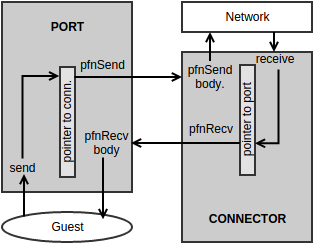
\includegraphics[scale=.75]{img/port_conn_if.png}
	 	\caption{Example of EMT execution flow}
	 	\label{img:port_conn_if}
\end{figure}
In this way, when a port wants to send a frame to the network, it invokes the \texttt{pfnBeginXmit} function provided by the connector in order to gain lock access on the connector itself; then it calls \texttt{pfnAllocBuf} function to get a buffer where the port can store the frame and, finally, it invokes \texttt{pfnSendBuf} so that the connector can push the frame (passed as argument) to the network.
On the other direction, when the connector gets a frame from the network, it invokes the \texttt{pfnWaitReceiveAvail} to whether the port is able to receive data. If this is the case, it immediately calls \texttt{pfnReceive} so that the port can push the received frame (passed as argument) to the guest.
\\
A simplified version of the above interaction is depicted in figure~\ref{img:port_conn_if}, where only the \textit{send} and \textit{receive} functions are shown.
\section{VirtualBox e1000 emulation}  \label{sec:e1000_emu}
The e1000\footnote{For detailed information about e1000 class of network adapters, refer to~\cite{e1000}} port is implemented in VirtualBox through three source files~\footnote{These source files are located in src/VBox/Devices/Network/ in the VirtualBox project root directory.}: \textit{DevE1000.cpp}, which is the one we are interested in, \textit{DevE1000Phy.cpp} and \textit{DevEEPROM.cpp}. The first one contains all the "emulation logic" part, while the others implement only the internal physical emulation and the internal EEPROM respectively. \subsection{TX emulation}
\subsection{RX emulation}
\chapter{Implementing netmap support}
\section{Initialization}
\section{Send side}
\section{Receive side}
\chapter{Optimizations on e1000 emulated device}
\section{Analysis of current implementation}
\subsection{TX performance}
\subsection{RX performance}
\section{Implementing mapping of descriptors}
\subsection{Implementation}
\subsection{Performance analysis}
\section{Packet batching}
\subsection{Implementation}
\subsection{Modification of netmap implementation}
\subsection{Performance analysis}
\chapter{Conclusions}

%\addcontentsline{toc}{section}{\refname}
\begin{thebibliography}{30}
\bibitem{vbox} VirtualBox project. \url{https://www.virtualbox.org}
\bibitem{netmap} \autori{Rizzo L.} \textit{netmap: a novel framework for fast packet I/O} \url{http://info.iet.unipi.it/~luigi/papers/20120503-netmap-atc12.pdf}
\bibitem{vale} \autori{Rizzo L., Lettieri G.} \textit{VALE: a switched ethernet for virtual machines.} \url{http://info.iet.unipi.it/~luigi/papers/20121026-vale.pdf}
\bibitem{amd-v} \autori{AMD} \textit{Secure Virtual Machine Architecture Reference Manual.}
\bibitem{vt-x} \autori{Neiger, Gil Santoni, A.} Intel virtualization technology: Hardware support for efficient processor virtualization. \textit{Intel Technology Journal 10, 3 (2006)}
\bibitem{iommu} \autori{Yehuda, B.} Utilizing IOMMUs for virtualization in linux and xen.
\bibitem{vmm_opt} \autori{Agensen, O., Mattson, J., Rugina, R., Sheldon, J.} Software techniques for avoiding hardware virtualization exits.
\bibitem{virtio} \autori{Russel, R.} virtio: towards a de-facto standard for virtual I/O devices.
\bibitem{rings} \autori{Intel} \textit{Intel 64 and IA-32 Architectures Software Developer's Manual}.
\bibitem{e1000} \autori{Intel} \textit{PCI/PCI-X Family of Gigabit Ethernet Controllers Software Developers Manual.}
\end{thebibliography}
	
\end{document}
